% ============================================================
%  SOLAR FILAMENT SEGMENTATION — SSN CSE PROJECT REPORT
% ============================================================
\documentclass[12pt,a4paper,openany]{report}
\usepackage[a4paper,top=1in,bottom=1in,left=1.25in,right=1in]{geometry}
\usepackage{times}
\usepackage{setspace}
\usepackage{titlesec}
\usepackage{graphicx}
\usepackage{amsmath,amssymb}
\usepackage{booktabs}
\usepackage{longtable}
\usepackage{enumitem}
\usepackage{fancyhdr}
\usepackage{hyperref}
\usepackage{xcolor}
\usepackage{listings}
\usepackage{caption}
\usepackage{tocloft}
\usepackage{parskip}
\usepackage{array}
\usepackage{tabularx}
\usepackage{tikz}
\usepackage{mdframed}
\usepackage{float}
\usepackage{microtype}
\usetikzlibrary{shapes.geometric,arrows.meta,positioning,calc,backgrounds}

\definecolor{ssnblue}{RGB}{0,56,101}
\definecolor{codebg}{rgb}{0.97,0.97,0.97}
\definecolor{codekw}{RGB}{0,0,160}
\definecolor{codecom}{RGB}{60,128,60}
\definecolor{codestr}{RGB}{160,0,0}
\definecolor{boxbg}{RGB}{240,245,255}
\definecolor{highlight}{RGB}{255,250,220}

\lstdefinestyle{pystyle}{
  backgroundcolor=\color{codebg},basicstyle=\ttfamily\small,
  keywordstyle=\color{codekw}\bfseries,commentstyle=\color{codecom}\itshape,
  stringstyle=\color{codestr},numberstyle=\tiny\color{gray},
  numbers=left,stepnumber=1,frame=single,rulecolor=\color{black!25},
  breaklines=true,showstringspaces=false,tabsize=4,language=Python,captionpos=b
}
\lstset{style=pystyle}

\pagestyle{fancy}
\fancyhf{}
\fancyhead[L]{\small\textit{Solar Filament Segmentation using YOLOv8l-Seg}}
\fancyhead[R]{\small\textit{SSN College of Engineering}}
\fancyfoot[C]{\thepage}
\renewcommand{\headrulewidth}{0.4pt}
\setlength{\headheight}{15pt}

% ============================================================
% TITLE FORMATTING — chapters and sections flow inline (no forced page breaks)
% ============================================================
\titleclass{\chapter}{straight}
\titleformat{\chapter}[block]
  {\normalfont\Large\bfseries\color{ssnblue}}{Chapter \thechapter:\ }{8pt}{}
\titleformat{name=\chapter,numberless}[block]
  {\normalfont\Large\bfseries\color{ssnblue}}{}{0pt}{}
\titlespacing*{\chapter}{0pt}{18pt}{8pt}
\titleformat{\section}{\normalfont\large\bfseries}{\thesection\quad}{6pt}{}
\titlespacing*{\section}{0pt}{14pt}{6pt}
\titleformat{\subsection}{\normalfont\normalsize\bfseries}{\thesubsection\quad}{6pt}{}
\titlespacing*{\subsection}{0pt}{10pt}{4pt}
\onehalfspacing

\hypersetup{colorlinks=true,linkcolor=ssnblue,urlcolor=blue!70!black,
  citecolor=green!40!black,
  pdftitle={Solar Filament Segmentation using YOLOv8l-Seg},pdfauthor={Boobathi}}

\tikzset{
  block/.style={rectangle,draw=ssnblue,thick,fill=boxbg,rounded corners=4pt,
    text width=5cm,align=center,minimum height=1cm,font=\small},
  sblock/.style={rectangle,draw=gray,thick,fill=white,rounded corners=3pt,
    text width=3.5cm,align=center,minimum height=0.8cm,font=\footnotesize},
  arrow/.style={-{Stealth[length=6pt]},thick,color=ssnblue},
  decision/.style={diamond,draw=orange!80!black,thick,fill=orange!15,aspect=2.8,
    text width=2.5cm,align=center,font=\footnotesize},
  term/.style={rectangle,draw=ssnblue,thick,fill=ssnblue!15,rounded corners=8pt,
    text width=5cm,align=center,minimum height=0.9cm,font=\small\bfseries}
}

\newmdenv[backgroundcolor=boxbg,linecolor=ssnblue,linewidth=1.5pt,
  roundcorner=4pt,innertopmargin=6pt,innerbottommargin=6pt,
  skipabove=8pt,skipbelow=8pt]{defbox}

\begin{document}

% ---- COVER PAGE ----
\begin{titlepage}
\centering
\vspace*{0.5cm}
{\large\textbf{Sri Sivasubramaniya Nadar College of Engineering}\\
Kalavakkam, Chennai -- 603 110\\
Department of Computer Science and Engineering}
\vspace{0.8cm}
\rule{\linewidth}{1.5pt}\vspace{0.4cm}
{\Huge\bfseries\color{ssnblue}Solar Filament Segmentation\\[6pt]using YOLOv8l-Seg\par}
\vspace{0.4cm}\rule{\linewidth}{0.8pt}\vspace{0.5cm}
{\large\itshape An End-to-End Instance Segmentation Pipeline\\
on the MAGFiLO 1.0 Dataset (Kaggle 2026)\\[4pt]
\textbf{Implementation: \texttt{solaris.py}}}
\vspace{1.2cm}
\begin{tabular}{rl}
\textbf{Submitted by:} & Boobathi \\[4pt]
\textbf{Degree:}       & B.E.\ Computer Science and Engineering \\[4pt]
\textbf{Date:}         & September 2026 \\
\end{tabular}
\vfill
\begin{mdframed}[backgroundcolor=ssnblue!10,linecolor=ssnblue,linewidth=1pt,roundcorner=4pt]
\centering\small
This report is submitted in partial fulfillment of the requirements\\
for the Bachelor of Engineering degree.
\end{mdframed}
\end{titlepage}

% ---- ABSTRACT ----
\chapter*{Abstract}
\addcontentsline{toc}{chapter}{Abstract}
\thispagestyle{fancy}
Solar filaments are dark, thread-like plasma clouds visible in H-alpha images of the Sun.
Their eruption can cause Coronal Mass Ejections (CMEs) that disrupt satellites, power grids,
and communication systems on Earth.

This report presents \textbf{Solaris}, an automated deep learning pipeline that detects and
segments solar filaments using \textbf{YOLOv8l-Seg}. The pipeline was trained on the
\textbf{MAGFiLO 1.0} dataset (Kaggle 2026 competition) and achieved a \textbf{Dice score
of 0.55}. It runs without code changes on Kaggle, Google Colab, and local machines.

The five pipeline stages are: (1)~environment detection, (2)~COCO-to-YOLO label conversion,
(3)~model training at $2048\times2048$, (4)~inference with overlap removal, and
(5)~RLE submission CSV generation.

\vspace{0.4cm}
\noindent\textbf{Keywords:} Solar Filament, Instance Segmentation, YOLOv8, COCO, RLE, MAGFiLO.

\tableofcontents
\listoffigures
\listoftables

% ========================================================
\chapter{Introduction to Solar Filaments}
% ========================================================

\section{The Sun and H-alpha Imaging}

The Sun is a giant ball of hot plasma. Its outer layer, the \textbf{chromosphere}, is studied
using \textbf{H-alpha light} (wavelength 656.3\,nm), which reveals structures invisible to
the naked eye. Telescopes fitted with H-alpha filters produce images where solar filaments
appear as dark, elongated structures.

\section{What is a Solar Filament?}

\begin{defbox}
\textbf{Definition:} A \textbf{solar filament} is a long, dense cloud of cooler plasma
($\approx$10{,}000\,K) suspended above the hotter surface ($\approx$5{,}500\,K) by magnetic
field lines. It appears \textbf{dark} in H-alpha images because it absorbs H-alpha light.
When seen at the solar limb, it glows bright and is called a \textbf{solar prominence}.
\end{defbox}

\begin{figure}[H]
\centering
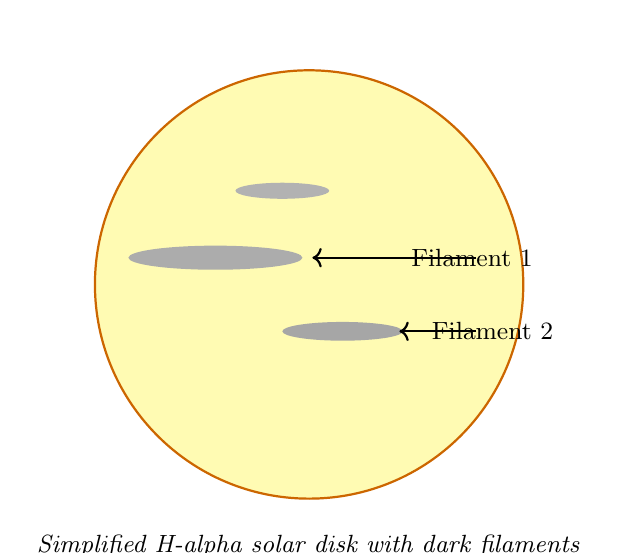
\begin{tikzpicture}[scale=0.85]
  \fill[yellow!30](0,0) circle(3.2cm);
  \draw[thick,orange!80!black](0,0) circle(3.2cm);
  \fill[gray!65](-1.4,0.4) ellipse(1.3cm and 0.18cm);
  \fill[gray!70](0.5,-0.7) ellipse(0.9cm and 0.14cm);
  \fill[gray!60](-0.4,1.4) ellipse(0.7cm and 0.12cm);
  \draw[->,thick](2.5,0.4)--(0.05,0.4)
    node[right,xshift=32pt,font=\small]{Filament 1};
  \draw[->,thick](2.5,-0.7)--(1.35,-0.7)
    node[right,xshift=8pt,font=\small]{Filament 2};
  \node[font=\small,below] at (0,-3.6)
    {\textit{Simplified H-alpha solar disk with dark filaments}};
\end{tikzpicture}
\caption{Solar filaments appear as dark elongated structures on an H-alpha solar disk image.}
\label{fig:halpha}
\end{figure}

\section{Importance of Filament Detection}

When a filament erupts, it can launch a \textbf{Coronal Mass Ejection (CME)} --- billions of
tonnes of plasma traveling toward Earth, capable of damaging satellites, disrupting GPS,
causing power grid failures, and endangering astronauts.

\begin{table}[H]
\centering
\caption{Applications of automated solar filament detection.}
\renewcommand{\arraystretch}{1.3}
\begin{tabular}{l p{9cm}}
\toprule
\textbf{Application} & \textbf{Benefit} \\
\midrule
Space-weather forecasting & Early warning for CME events \\
Satellite operations      & Adjust orientation before solar storms \\
Power grid management     & Pre-emptive load shedding \\
Scientific research       & Morphological study across decades of data \\
Astronaut safety          & Radiation advisories during EVAs \\
\bottomrule
\end{tabular}
\label{tab:apps}
\end{table}

% ========================================================
\chapter{Problem Statement and Objectives}
% ========================================================

\section{Limitations of Manual Annotation}

Historically, solar physicists manually examine images and draw filament boundaries.
This is: (1) \textbf{slow} (few images/hour), (2) \textbf{inconsistent} (subjective),
(3) \textbf{unscalable} (millions of images exist), and (4) \textbf{error-prone}.

\section{Project Objectives}

\begin{enumerate}[label=\textbf{O\arabic*.}]
  \item Build an automated pipeline for pixel-accurate filament instance segmentation.
  \item Use \textbf{YOLOv8l-Seg} trained on \textbf{MAGFiLO 1.0} (Kaggle 2026).
  \item Generate a competition-ready \texttt{submission.csv} in COCO RLE format.
  \item Make the pipeline portable: Kaggle, Colab, local --- same code, no changes.
\end{enumerate}

\section{System Overview}

\begin{figure}[H]
\centering
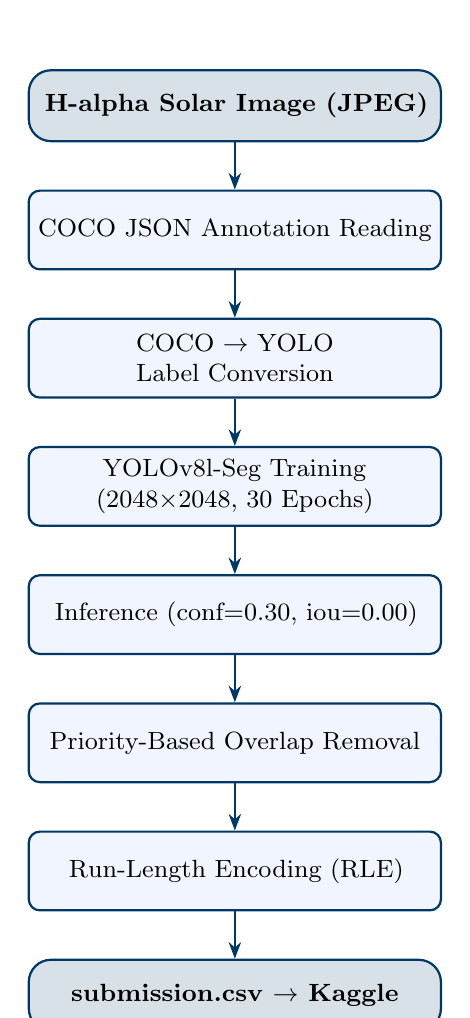
\begin{tikzpicture}[node distance=0.6cm]
  \node[term](inp){H-alpha Solar Image (JPEG)};
  \node[block,below=of inp](coco){COCO JSON Annotation Reading};
  \node[block,below=of coco](conv){COCO $\to$ YOLO Label Conversion};
  \node[block,below=of conv](train){YOLOv8l-Seg Training\\(2048$\times$2048, 30 Epochs)};
  \node[block,below=of train](infer){Inference (conf=0.30, iou=0.00)};
  \node[block,below=of infer](ovlp){Priority-Based Overlap Removal};
  \node[block,below=of ovlp](rle){Run-Length Encoding (RLE)};
  \node[term,below=of rle](out){submission.csv $\to$ Kaggle};
  \foreach \a/\b in {inp/coco,coco/conv,conv/train,
                     train/infer,infer/ovlp,ovlp/rle,rle/out}
    \draw[arrow](\a)--(\b);
\end{tikzpicture}
\caption{Complete end-to-end Solaris pipeline from raw image to Kaggle submission.}
\label{fig:overview}
\end{figure}

% ========================================================
\chapter{Dataset: MAGFiLO 1.0}
% ========================================================

\section{Dataset Overview}

\textbf{MAGFiLO} (MAGnetic Filaments LOcalization) is a curated H-alpha solar image
dataset with expert filament annotations. It was provided in the Kaggle 2026 competition
\texttt{filament-segmentation-2026}.

\begin{lstlisting}[language=bash,style=pystyle,
  caption={MAGFiLO dataset directory structure.}]
filament-segmentation-2026/
 L-- MAGFiLO_1.0_Kaggle_2026/
      |-- train_images/          # Labeled training images
      |-- test_images/           # Unlabeled test images
      L-- Annotations/
           L-- Annotations_train.json  # COCO labels
\end{lstlisting}

\begin{table}[H]
\centering
\caption{MAGFiLO 1.0 dataset key statistics.}
\renewcommand{\arraystretch}{1.3}
\begin{tabular}{l l}
\toprule
\textbf{Property}   & \textbf{Value} \\
\midrule
Image type          & Full-disk H-alpha solar images \\
Image format        & JPEG \\
Annotation format   & COCO JSON \\
Object class        & 1 (filament, class ID = 0) \\
Annotation types    & Polygon coordinates and RLE dictionary \\
Train/Val split     & 90\% train, 10\% val (random seed=42) \\
\bottomrule
\end{tabular}
\label{tab:dataset}
\end{table}

\section{Path Auto-Detection Flowchart}

\begin{figure}[H]
\centering
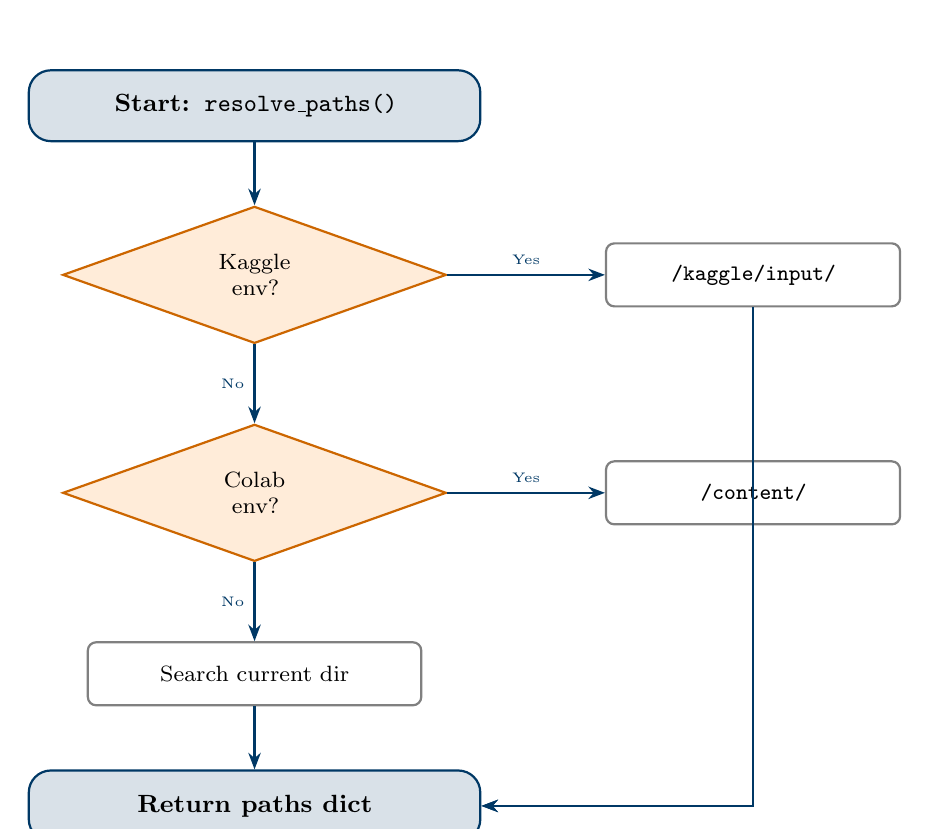
\begin{tikzpicture}[node distance=0.6cm]
  \node[term,text width=5.5cm](s){Start: \texttt{resolve\_paths()}};
  \node[decision,below=0.8cm of s](k){Kaggle\\env?};
  \node[sblock,right=2cm of k](kp){\texttt{/kaggle/input/}};
  \node[decision,below=1cm of k](c){Colab\\env?};
  \node[sblock,right=2cm of c](cp){\texttt{/content/}};
  \node[sblock,below=1cm of c,text width=4cm](lp){Search current dir};
  \node[term,below=0.8cm of lp,text width=5.5cm](e){Return paths dict};
  \draw[arrow](s)--(k);
  \draw[arrow](k)--node[above,font=\tiny]{Yes}(kp);
  \draw[arrow](k)--node[left,font=\tiny]{No}(c);
  \draw[arrow](c)--node[above,font=\tiny]{Yes}(cp);
  \draw[arrow](c)--node[left,font=\tiny]{No}(lp);
  \draw[arrow](lp)--(e);
  \draw[arrow](kp)|-(e);
  \draw[arrow](cp)|-(e);
\end{tikzpicture}
\caption{Flowchart of \texttt{resolve\_paths()} environment auto-detection.}
\label{fig:resolve}
\end{figure}

% ========================================================
\chapter{COCO JSON Annotation Format}
% ========================================================

\section{Structure of a COCO File}

COCO (Common Objects in Context) is an industry-standard JSON annotation format
with three top-level arrays:

\begin{table}[H]
\centering
\caption{Top-level sections of a COCO JSON file.}
\renewcommand{\arraystretch}{1.3}
\begin{tabular}{l p{9cm}}
\toprule
\textbf{Key} & \textbf{Meaning} \\
\midrule
\texttt{images}      & List of all images: ID, filename, width, height \\
\texttt{annotations} & List of all labeled objects; each entry = one filament \\
\texttt{categories}  & Class names; for MAGFiLO: only \texttt{filament} (ID=1) \\
\bottomrule
\end{tabular}
\label{tab:coco_top}
\end{table}

\section{Annotation Field Reference}

\begin{lstlisting}[caption={Complete COCO annotation entry example.}]
{
  "id": 101,           /* Unique annotation ID          */
  "image_id": 42,      /* Links to images[id==42]       */
  "category_id": 1,    /* 1 = filament class            */
  "segmentation": [[120.5, 80.3, 135.0, 82.1,
                    140.2, 90.5, 125.0, 91.0]],
  "bbox": [120.5, 80.3, 19.7, 10.7],  /* [x,y,w,h]     */
  "area": 180.5,
  "iscrowd": 0
}
\end{lstlisting}

\begin{table}[H]
\centering
\caption{Detailed COCO annotation field explanations.}
\renewcommand{\arraystretch}{1.3}
\begin{tabular}{l l p{7cm}}
\toprule
\textbf{Field} & \textbf{Type} & \textbf{Meaning} \\
\midrule
\texttt{id}           & integer & Unique ID of this annotation \\
\texttt{image\_id}    & integer & Links to image via \texttt{images.id} \\
\texttt{category\_id} & integer & Class (1 = filament) \\
\texttt{segmentation} & list/dict & Polygon coords OR RLE dict \\
\texttt{bbox}         & list    & Bounding box [x,y,width,height] \\
\texttt{area}         & float   & Pixel count inside polygon \\
\texttt{iscrowd}      & 0 or 1  & 0 = individual instance \\
\bottomrule
\end{tabular}
\label{tab:coco_ann}
\end{table}

\section{Two Segmentation Encoding Types}

\begin{defbox}
\textbf{Polygon List:} A list of $(x,y)$ pixel coordinates tracing the boundary.
Minimum 3 points (6 values). Example: \texttt{[[x1,y1,x2,y2,...,xn,yn]]}

\vspace{4pt}
\textbf{RLE Dictionary:} Compressed mask with \texttt{counts} (bytes) and \texttt{size}
[height, width]. Used when masks are computed rather than hand-drawn.
\end{defbox}

\section{Polygon Coordinate System}

\begin{figure}[H]
\centering
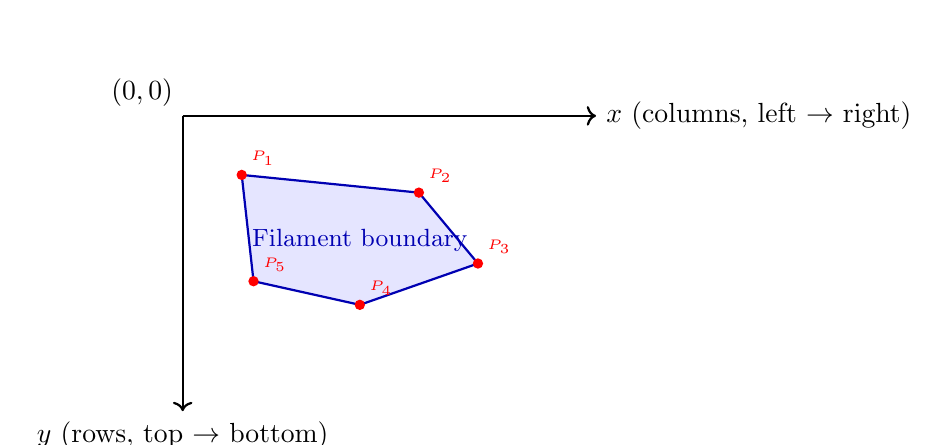
\begin{tikzpicture}[scale=0.75]
  \draw[thick,->](0,0)--(7,0)
    node[right]{$x$ (columns, left $\to$ right)};
  \draw[thick,->](0,0)--(0,-5)
    node[below]{$y$ (rows, top $\to$ bottom)};
  \node[above left] at (0,0){$(0,0)$};
  \fill[blue!20,opacity=0.5]
    (1,-1)--(4,-1.3)--(5,-2.5)--(3,-3.2)--(1.2,-2.8)--cycle;
  \draw[thick,blue!70!black]
    (1,-1)--(4,-1.3)--(5,-2.5)--(3,-3.2)--(1.2,-2.8)--cycle;
  \foreach \p/\l in {(1,-1)/$P_1$,(4,-1.3)/$P_2$,(5,-2.5)/$P_3$,
                     (3,-3.2)/$P_4$,(1.2,-2.8)/$P_5$}
    \fill[red]\p circle(2.5pt) node[above right,font=\tiny]{\l};
  \node[blue!70!black,font=\small] at (3,-2.1){Filament boundary};
\end{tikzpicture}
\caption{Polygon coordinate system. Origin is top-left; $x$ increases right, $y$ downward.}
\label{fig:polygon}
\end{figure}

% ========================================================
\chapter{COCO to YOLO Label Conversion}
% ========================================================

\section{Why Convert?}

YOLOv8-Seg cannot read COCO JSON. It requires one plain-text \texttt{.txt} label file per
image with normalized coordinates.

\section{YOLO Label Format and Normalization}

Each line in a YOLO label file represents one filament:
\begin{lstlisting}[language=bash,caption={YOLO segmentation label format.}]
<class_id> x1 y1 x2 y2 ... xn yn   (all normalized to [0,1])
\end{lstlisting}

Normalization formula:
\begin{equation}
  x_{\text{norm}} = \frac{x_{\text{pixel}}}{W},\qquad
  y_{\text{norm}} = \frac{y_{\text{pixel}}}{H}
  \label{eq:norm}
\end{equation}

\textbf{Example:} Image $1280\times960$, pixel $(640,480) \to (0.5000, 0.5000)$.

\begin{table}[H]
\centering
\caption{COCO vs.\ YOLO format comparison.}
\renewcommand{\arraystretch}{1.3}
\begin{tabular}{l p{4.8cm} p{4.8cm}}
\toprule
\textbf{Property} & \textbf{COCO JSON} & \textbf{YOLO TXT} \\
\midrule
Format      & JSON                & Plain text \\
File scope  & One JSON all images & One \texttt{.txt} per image \\
Coordinates & Pixel values        & Normalized $[0,1]$ \\
RLE support & Yes                 & No (decoded to polygon) \\
\bottomrule
\end{tabular}
\label{tab:cocovsyolo}
\end{table}

\section{Conversion Flowchart}

\begin{figure}[H]
\centering
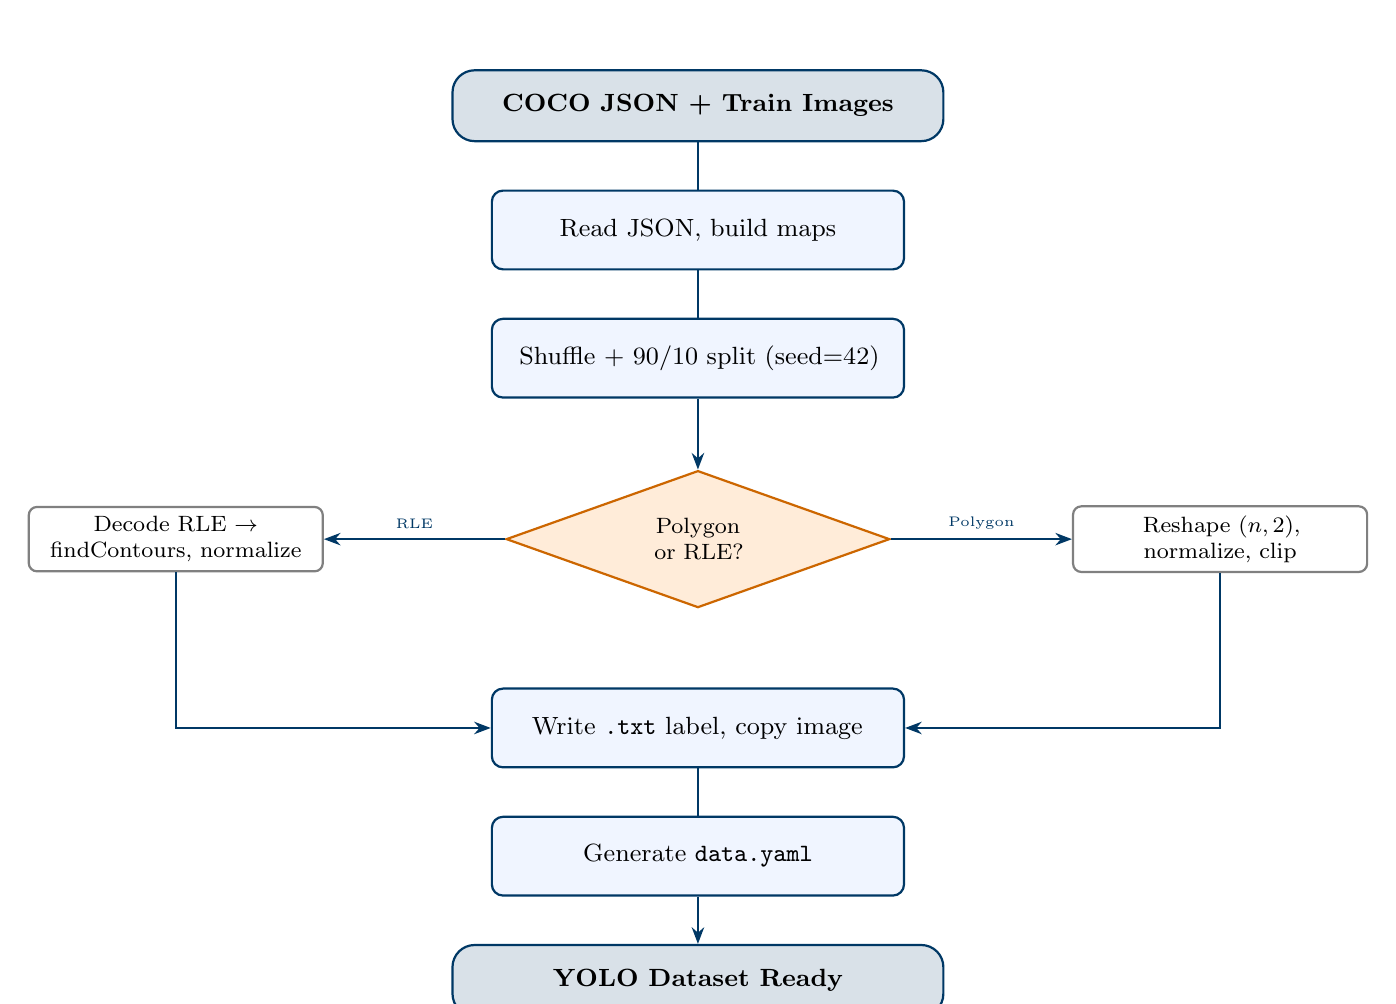
\begin{tikzpicture}[node distance=0.6cm]
  \node[term,text width=6cm](in){COCO JSON + Train Images};
  \node[block,below=of in](read){Read JSON, build maps};
  \node[block,below=of read](split){Shuffle + 90/10 split (seed=42)};
  \node[decision,below=0.9cm of split](type){Polygon\\or RLE?};
  \node[sblock,right=2.3cm of type](poly){Reshape $(n,2)$,\\normalize, clip};
  \node[sblock,left=2.3cm of type](rle){Decode RLE $\to$\\findContours, normalize};
  \node[block,below=1cm of type](write){Write \texttt{.txt} label, copy image};
  \node[block,below=of write](yaml){Generate \texttt{data.yaml}};
  \node[term,below=of yaml,text width=6cm](out){YOLO Dataset Ready};
  \draw[arrow](in)--(read)--(split)--(type);
  \draw[arrow](type)--node[above,font=\tiny]{Polygon}(poly);
  \draw[arrow](type)--node[above,font=\tiny]{RLE}(rle);
  \draw[arrow](poly)|-(write);
  \draw[arrow](rle)|-(write);
  \draw[arrow](write)--(yaml)--(out);
\end{tikzpicture}
\caption{Flowchart of the \texttt{convert\_coco\_to\_yolo\_seg()} function.}
\label{fig:convert}
\end{figure}

% ========================================================
\chapter{Image Preprocessing Pipeline}
% ========================================================

\section{Resizing to $2048\times2048$}

\begin{defbox}
\textbf{Why 2048 px?} Filaments are thin. At YOLO's default 640 px, fine detail is lost.
Training at 2048 px preserves thread-like structure for accurate detection.
\end{defbox}

YOLOv8 uses \textbf{letterboxing}: scale image to fit $2048\times2048$ maintaining aspect
ratio; pad remaining area with grey (value 114).

\section{Pixel Normalization}

\begin{equation}
  p_{\text{norm}} = p_{\text{pixel}} / 255
  \label{eq:pixnorm}
\end{equation}

Scales pixel values from $[0,255]$ to $[0,1]$ for stable gradient optimization.

\section{Data Augmentation}

\begin{table}[H]
\centering
\caption{Data augmentation operations in Solaris training.}
\renewcommand{\arraystretch}{1.3}
\begin{tabular}{l c p{7cm}}
\toprule
\textbf{Augmentation} & \textbf{Probability} & \textbf{Justification} \\
\midrule
Horizontal flip & 50\% & Filaments appear in any orientation; teaches symmetry \\
Vertical flip   & 50\% & Solar disk has no ``up''; physically valid transformation \\
Mosaic          & 50\% & Stitches 4 images; exposes model to varied scales \\
\bottomrule
\end{tabular}
\label{tab:aug}
\end{table}

\begin{figure}[H]
\centering
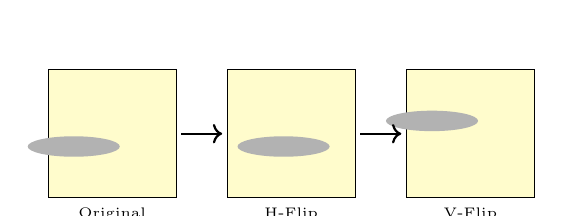
\begin{tikzpicture}[scale=0.65]
  \draw[fill=yellow!20,draw=black](0,0) rectangle(2.5,2.5);
  \fill[gray!60](0.5,1.0) ellipse(0.9 and 0.2);
  \node[font=\tiny,below] at (1.25,0){Original};
  \draw[fill=yellow!20,draw=black](3.5,0) rectangle(6,2.5);
  \fill[gray!60](4.6,1.0) ellipse(0.9 and 0.2);
  \node[font=\tiny,below] at (4.75,0){H-Flip};
  \draw[fill=yellow!20,draw=black](7,0) rectangle(9.5,2.5);
  \fill[gray!60](7.5,1.5) ellipse(0.9 and 0.2);
  \node[font=\tiny,below] at (8.25,0){V-Flip};
  \draw[->,thick](2.6,1.25)--(3.4,1.25);
  \draw[->,thick](6.1,1.25)--(6.9,1.25);
\end{tikzpicture}
\caption{Horizontal and vertical flip augmentations applied to a solar image example.}
\label{fig:augment}
\end{figure}

\begin{table}[H]
\centering
\caption{Image preprocessing pipeline steps.}
\renewcommand{\arraystretch}{1.3}
\begin{tabular}{c l l}
\toprule
\textbf{Step} & \textbf{Operation} & \textbf{Result} \\
\midrule
1 & Read JPEG         & Raw array $(H,W,3)$ \\
2 & Letterbox resize  & $2048\times2048\times3$ \\
3 & Normalize pixels  & Values in $[0,1]$ \\
4 & Tensor convert    & PyTorch tensor \\
5 & Batch stack       & $(B,3,2048,2048)$ \\
6 & Augmentation      & Flips and mosaic \\
\bottomrule
\end{tabular}
\label{tab:preproc}
\end{table}

% ========================================================
\chapter{YOLOv8l-Seg Architecture}
% ========================================================

\section{YOLO Overview}

YOLO (You Only Look Once) processes the entire image in one pass, simultaneously predicting
all object locations and shapes. YOLOv8 (Ultralytics, 2023) is the current state-of-the-art.

\begin{table}[H]
\centering
\caption{YOLOv8 segmentation model variants.}
\renewcommand{\arraystretch}{1.3}
\begin{tabular}{l r r r}
\toprule
\textbf{Variant} & \textbf{Parameters} & \textbf{Speed} & \textbf{Accuracy} \\
\midrule
YOLOv8n-seg &  3.4\,M & Very Fast & Low     \\
YOLOv8s-seg & 11.8\,M & Fast      & Medium  \\
YOLOv8m-seg & 27.3\,M & Moderate  & Good    \\
\textbf{YOLOv8l-seg} & \textbf{46.0\,M} & Slower & \textbf{High} \\
YOLOv8x-seg & 71.8\,M & Slowest   & Highest \\
\bottomrule
\end{tabular}
\label{tab:yolo_variants}
\end{table}

\section{Why YOLOv8l-Seg?}

Filaments are thin, low-contrast structures. The Large variant's deeper backbone provides
higher representational capacity. ``Seg'' outputs pixel-accurate masks, not just boxes.

\section{Three Main Blocks}

\textbf{Backbone (CSPDarknet):} Extracts hierarchical features from the image. Spatial
resolution decreases, channel depth increases, and the network learns progressively more
abstract representations.

\textbf{Neck (PAN-FPN):} Combines feature maps from multiple backbone levels bidirectionally,
giving the head access to both fine detail (shallow) and broad context (deep).

\textbf{Head:} Produces bounding boxes, class scores, 32 shared prototype masks, and
per-instance mask coefficients. The final instance mask is:

\begin{equation}
  M_i = \sigma\!\left(\sum_{k=1}^{32} c_{i,k} \cdot P_k\right)
  \label{eq:mask}
\end{equation}

where $P_k$ are shared prototypes, $c_{i,k}$ are instance weights, $\sigma$ is sigmoid.

\begin{figure}[H]
\centering
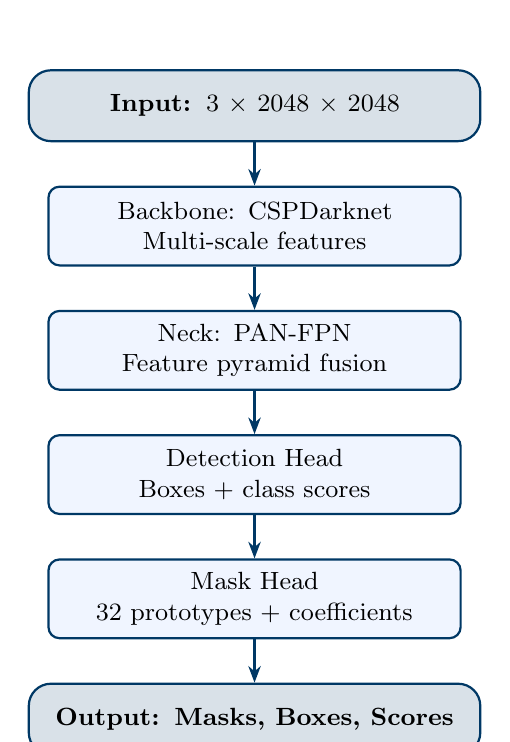
\begin{tikzpicture}[node distance=0.55cm]
  \node[term,text width=5.5cm](img){Input: $3\times2048\times2048$};
  \node[block,below=of img](b1){Backbone: CSPDarknet\\Multi-scale features};
  \node[block,below=of b1](neck){Neck: PAN-FPN\\Feature pyramid fusion};
  \node[block,below=of neck](det){Detection Head\\Boxes + class scores};
  \node[block,below=of det](seg){Mask Head\\32 prototypes + coefficients};
  \node[term,below=of seg,text width=5.5cm](out){Output: Masks, Boxes, Scores};
  \foreach \a/\b in {img/b1,b1/neck,neck/det,det/seg,seg/out}
    \draw[arrow](\a)--(\b);
\end{tikzpicture}
\caption{Simplified YOLOv8l-Seg architecture showing information flow from image to output.}
\label{fig:arch}
\end{figure}

% ========================================================
\chapter{Complete Training Pipeline}
% ========================================================

\section{Training Workflow}

\textbf{Step 1 --- Read image and label:} Load one image and its YOLO \texttt{.txt} label.

\textbf{Step 2 --- Rasterize polygon:} Convert polygon boundary to a binary ground-truth mask.

\textbf{Step 3 --- Forward pass:} Image passes through backbone, neck, head; model
generates a predicted mask.

\textbf{Step 4 --- Compute loss:} Compare prediction to ground truth using composite loss.

\textbf{Step 5 --- Backpropagation:} Error flows backward; weights are adjusted by AdamW.

\textbf{Step 6 --- Repeat for one epoch:} Steps 1--5 for all training images (30 epochs total).

\section{Loss Function}

\begin{equation}
  \mathcal{L}_{\text{total}}
  = \lambda_\text{box}\mathcal{L}_\text{box}
  + \lambda_\text{cls}\mathcal{L}_\text{cls}
  + \lambda_\text{dfl}\mathcal{L}_\text{dfl}
  + \lambda_\text{mask}\mathcal{L}_\text{mask}
  \label{eq:loss}
\end{equation}

\begin{table}[H]
\centering
\caption{Components of the YOLOv8 composite loss function.}
\renewcommand{\arraystretch}{1.3}
\begin{tabular}{l p{9cm}}
\toprule
\textbf{Component} & \textbf{Meaning} \\
\midrule
$\mathcal{L}_\text{box}$  & Error in predicted bounding box position/size \\
$\mathcal{L}_\text{cls}$  & Error in class confidence score \\
$\mathcal{L}_\text{dfl}$  & Distribution Focal Loss for precise coordinate regression \\
$\mathcal{L}_\text{mask}$ & Per-pixel binary cross-entropy between predicted and true mask \\
\bottomrule
\end{tabular}
\label{tab:loss}
\end{table}

\section{Training Hyperparameters}

\begin{table}[H]
\centering
\caption{Training hyperparameters used in \texttt{solaris.py}.}
\renewcommand{\arraystretch}{1.3}
\begin{tabular}{l l p{7cm}}
\toprule
\textbf{Parameter} & \textbf{Value} & \textbf{Reason} \\
\midrule
\texttt{epochs}    & 30    & Complete passes over training data \\
\texttt{imgsz}     & 2048  & Preserve thin filament structures \\
\texttt{batch}     & 2     & GPU memory constraint at 2048px \\
\texttt{optimizer} & AdamW & Stable convergence, weight decay \\
\texttt{lr0}       & 0.001 & Initial learning rate \\
\texttt{lrf}       & 0.01  & Final LR: $0.01\times$lr0, cosine decay \\
\texttt{mosaic}    & 0.5   & 50\% mosaic augmentation \\
\texttt{fliplr}    & 0.5   & 50\% horizontal flip \\
\texttt{flipud}    & 0.5   & 50\% vertical flip \\
\bottomrule
\end{tabular}
\label{tab:hyperparam}
\end{table}

\section{Model Checkpointing}

\begin{table}[H]
\centering
\caption{Checkpoint files saved during training.}
\renewcommand{\arraystretch}{1.3}
\begin{tabular}{l l p{7cm}}
\toprule
\textbf{File} & \textbf{Saved When} & \textbf{Meaning} \\
\midrule
\texttt{last.pt} & After every epoch  & Most recent weights \\
\texttt{best.pt} & When val mAP peaks & Best weights (used for inference) \\
\bottomrule
\end{tabular}
\label{tab:checkpoint}
\end{table}

% ========================================================
\chapter{Binary Masks and Segmentation}
% ========================================================

\section{Semantic vs.\ Instance Segmentation}

\begin{defbox}
\textbf{Semantic Segmentation:} Labels every pixel with a class but does NOT separate
individual objects. All filaments share the same colour.

\vspace{4pt}
\textbf{Instance Segmentation:} Labels every pixel AND separates each individual object.
Filament 1 and Filament 2 each get their own distinct mask. Required here because each
filament must be encoded separately in the Kaggle submission.
\end{defbox}

\section{Binary Mask}

A binary mask is a 2D matrix (same size as the image):
value \textbf{1} = filament pixel; value \textbf{0} = background pixel.

\begin{figure}[H]
\centering
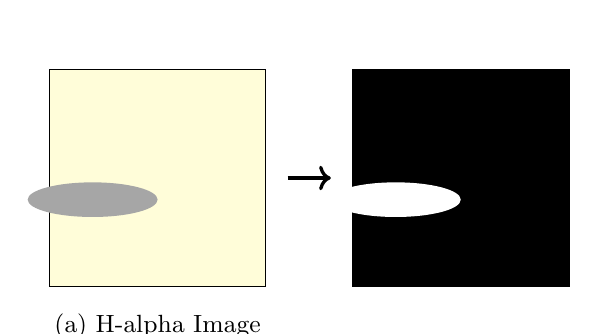
\begin{tikzpicture}[scale=0.55]
  \draw[fill=yellow!15,draw=black](0,0) rectangle(5,5);
  \fill[gray!70](1,2) ellipse(1.5 and 0.4);
  \node[font=\small,below] at (2.5,-0.4){(a) H-alpha Image};
  \draw[->,very thick](5.5,2.5)--(6.5,2.5);
  \draw[fill=black,draw=black](7,0) rectangle(12,5);
  \fill[white](8,2) ellipse(1.5 and 0.4);
  \node[white,font=\small,below] at (9.5,-0.4){(b) Binary Mask};
\end{tikzpicture}
\caption{Converting H-alpha image to binary mask. White (1) = filament; black (0) = background.}
\label{fig:binmask}
\end{figure}

Binary mask matrix example ($5\times5$, filament in row 3):
\[
\text{Mask} = \begin{pmatrix}
0 & 0 & 0 & 0 & 0 \\
0 & 0 & 0 & 0 & 0 \\
0 & 1 & 1 & 1 & 0 \\
0 & 0 & 0 & 0 & 0 \\
0 & 0 & 0 & 0 & 0
\end{pmatrix}
\]

\begin{table}[H]
\centering
\caption{Comparison of three object annotation formats.}
\renewcommand{\arraystretch}{1.3}
\begin{tabular}{l p{3.2cm} p{3.2cm} p{3.2cm}}
\toprule
\textbf{Property} & \textbf{Bounding Box} & \textbf{Polygon} & \textbf{Binary Mask} \\
\midrule
Shape       & Rectangle    & Boundary points & Per-pixel label \\
Precision   & Low          & Medium          & Pixel-perfect \\
Storage     & 4 numbers    & $2n$ numbers    & $H\times W$ matrix \\
\bottomrule
\end{tabular}
\label{tab:annformat}
\end{table}

% ========================================================
\chapter{Dice Score, Dice Loss, and IoU}
% ========================================================

\section{Building Blocks: TP, FP, FN}

Let $A$ = predicted mask, $B$ = ground truth mask:
\begin{itemize}
  \item \textbf{TP} = $|A\cap B|$: pixels predicted AND actually filament.
  \item \textbf{FP}: predicted filament but NOT actually filament.
  \item \textbf{FN}: actually filament but NOT predicted.
\end{itemize}

\section{Dice Score}

\begin{equation}
  \text{Dice} = \frac{2|A\cap B|}{|A|+|B|}
              = \frac{2\,\text{TP}}{2\,\text{TP}+\text{FP}+\text{FN}}
  \label{eq:dice}
\end{equation}

\textbf{Solaris achieved Dice = 0.55 on the Kaggle public leaderboard.}

\section{Dice Loss}

\begin{equation}
  \mathcal{L}_\text{Dice} = 1 - \text{Dice}
  \label{eq:diceloss}
\end{equation}

\section{Intersection over Union}

\begin{equation}
  \text{IoU} = \frac{|A\cap B|}{|A\cup B|}
             = \frac{\text{TP}}{\text{TP}+\text{FP}+\text{FN}}
  \label{eq:iou}
\end{equation}

\section{Relationship}

\begin{equation}
  \text{Dice} = \frac{2\,\text{IoU}}{1+\text{IoU}}
  \label{eq:dice_iou}
\end{equation}

Dice is always higher than IoU for the same prediction.

\section{Worked Example}

Given $|A|=50$, $|B|=60$, $|A\cap B|=40$:
\begin{align*}
  \text{TP}&=40,\;\text{FP}=10,\;\text{FN}=20\\
  \text{Dice}&=80/110\approx0.727\qquad
  \text{IoU}=40/70\approx0.571
\end{align*}

\begin{figure}[H]
\centering
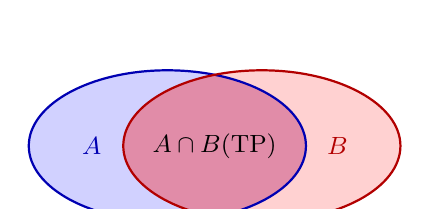
\begin{tikzpicture}[scale=0.8]
  \fill[blue!30,opacity=0.6](0,0) ellipse(2.2cm and 1.2cm);
  \fill[red!30,opacity=0.6](1.5,0) ellipse(2.2cm and 1.2cm);
  \begin{scope}
    \clip(0,0) ellipse(2.2cm and 1.2cm);
    \fill[purple!50,opacity=0.8](1.5,0) ellipse(2.2cm and 1.2cm);
  \end{scope}
  \draw[thick,blue!70!black](0,0) ellipse(2.2cm and 1.2cm);
  \draw[thick,red!70!black](1.5,0) ellipse(2.2cm and 1.2cm);
  \node[font=\small,blue!70!black] at (-1.2,0){$A$};
  \node[font=\small,red!70!black] at (2.7,0){$B$};
  \node[font=\small] at (0.75,0){$A\cap B$\\(TP)};
\end{tikzpicture}
\caption{Overlap of predicted mask $A$ and ground-truth $B$. Purple = true positive pixels.}
\label{fig:overlap}
\end{figure}

\begin{table}[H]
\centering
\caption{Comparison of Dice and IoU metrics.}
\renewcommand{\arraystretch}{1.3}
\begin{tabular}{l l l}
\toprule
\textbf{Property}  & \textbf{Dice} & \textbf{IoU} \\
\midrule
Formula            & $\frac{2|A\cap B|}{|A|+|B|}$ & $\frac{|A\cap B|}{|A\cup B|}$ \\
Range              & 0--1 & 0--1 \\
Kaggle metric used & \textbf{Yes} & No \\
Solaris result     & \textbf{0.55} & $\approx$0.38 \\
\bottomrule
\end{tabular}
\label{tab:dice_iou}
\end{table}

% ========================================================
\chapter{Prediction Pipeline}
% ========================================================

\section{Step-by-Step Inference}

\begin{enumerate}
  \item Load \texttt{best.pt} weights.
  \item Read test image in grayscale (capture $H,W$).
  \item Call \texttt{model.predict(img, imgsz=2048, conf=0.30, iou=0.00, max\_det=100)}.
  \item Extract raw mask tensor $(N,H_m,W_m)$ and confidence scores.
  \item Apply \texttt{remove\_instance\_overlaps()} for disjoint masks.
  \item Resize each mask to original $(W,H)$ using \texttt{INTER\_NEAREST}.
  \item Discard masks with fewer than 5 foreground pixels.
  \item RLE encode each mask; append row to \texttt{submission.csv}.
\end{enumerate}

\begin{table}[H]
\centering
\caption{Inference parameter settings and effects.}
\renewcommand{\arraystretch}{1.3}
\begin{tabular}{l l p{7.5cm}}
\toprule
\textbf{Parameter} & \textbf{Value} & \textbf{Effect} \\
\midrule
\texttt{imgsz}    & 2048 & Match training resolution \\
\texttt{conf}     & 0.30 & Keep detections with $\geq30\%$ confidence \\
\texttt{iou}      & 0.00 & Any box overlap triggers NMS suppression \\
\texttt{max\_det} & 100  & Max filaments per image \\
\bottomrule
\end{tabular}
\label{tab:infer_params}
\end{table}

\section{Priority Overlap Removal}

\begin{figure}[H]
\centering
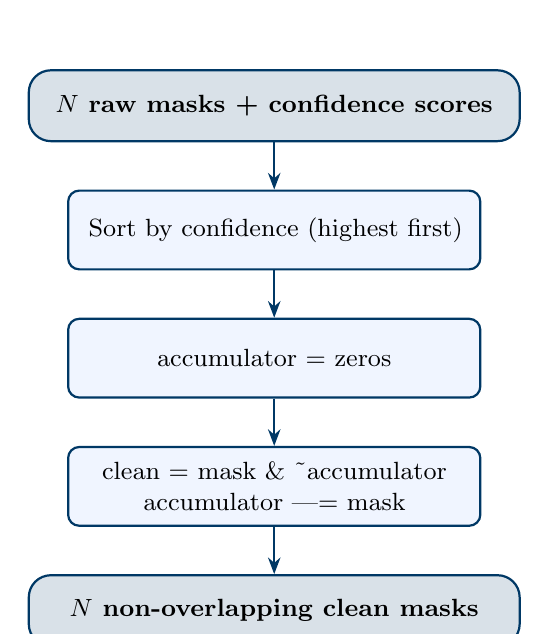
\begin{tikzpicture}[node distance=0.6cm]
  \node[term,text width=6cm](in){$N$ raw masks + confidence scores};
  \node[block,below=of in](sort){Sort by confidence (highest first)};
  \node[block,below=of sort](acc){accumulator = zeros};
  \node[block,below=of acc](loop){clean = mask \& \textasciitilde accumulator\\accumulator |= mask};
  \node[term,below=of loop,text width=6cm](out){$N$ non-overlapping clean masks};
  \foreach \a/\b in {in/sort,sort/acc,acc/loop,loop/out}
    \draw[arrow](\a)--(\b);
\end{tikzpicture}
\caption{Priority-based overlap removal: high-confidence masks claim pixels first.}
\label{fig:overlap_flow}
\end{figure}

% ========================================================
\chapter{Run-Length Encoding}
% ========================================================

\section{What is RLE?}

Instead of storing every pixel, RLE records how many consecutive zeros and ones appear:

\begin{defbox}
\textbf{Example:} Flat mask \texttt{0 0 0 1 1 1 0 0 1 1 0}\\
RLE: ``3 zeros, 3 ones, 2 zeros, 2 ones, 1 zero'' $\to$ encodes 11 values as 5 numbers.
\end{defbox}

COCO scans in \textbf{column-major (Fortran) order}. The \texttt{np.asfortranarray()} call
reorders memory before encoding.

\section{The Encoding Function}

\begin{lstlisting}[caption={mask\_to\_rle() from solaris.py.}]
def mask_to_rle(binary_mask):
    rle = mask_utils.encode(
        np.asfortranarray(binary_mask.astype(np.uint8)))
    rle["counts"] = rle["counts"].decode("utf-8")
    return rle["counts"]
\end{lstlisting}

\section{submission.csv Format}

\begin{table}[H]
\centering
\caption{Column format of the Kaggle submission CSV.}
\renewcommand{\arraystretch}{1.3}
\begin{tabular}{l l p{7cm}}
\toprule
\textbf{Column} & \textbf{Example} & \textbf{Meaning} \\
\midrule
\texttt{filament\_id}      & \texttt{img\_0042\_3} & Image stem + instance index \\
\texttt{segmentation\_rle} & \texttt{NjoxOTkw...}  & COCO RLE-encoded binary mask \\
\bottomrule
\end{tabular}
\label{tab:csv}
\end{table}

\begin{figure}[H]
\centering
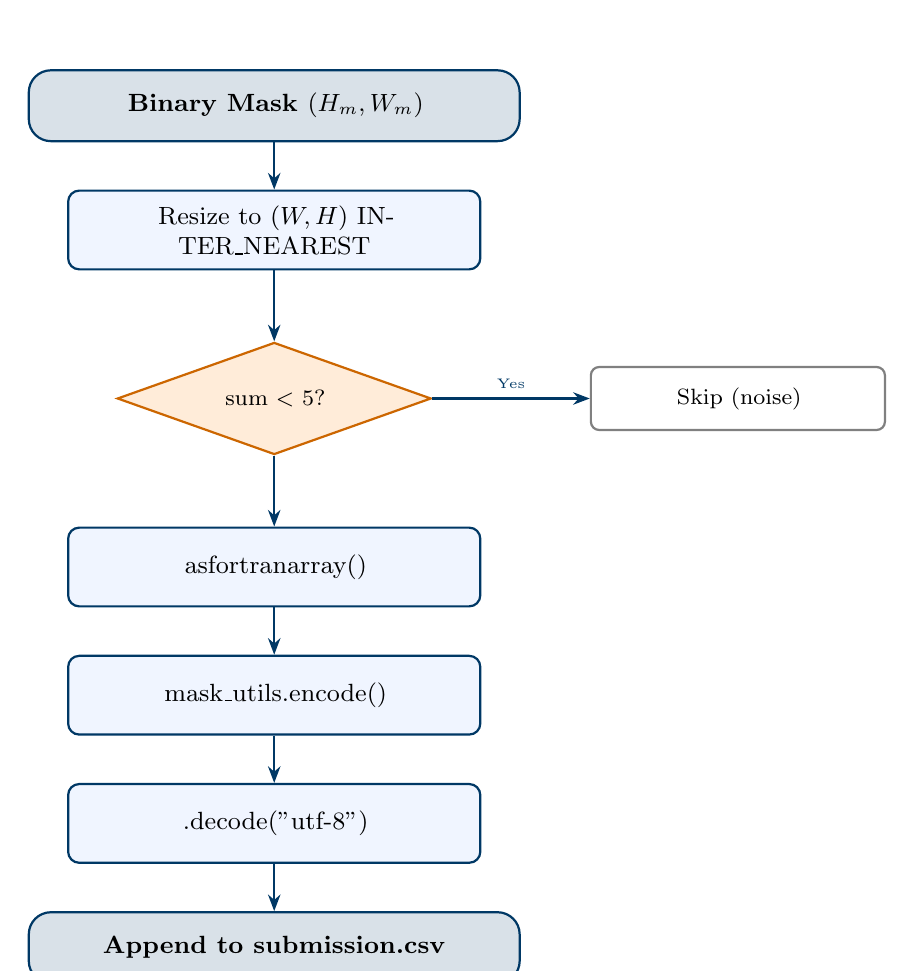
\begin{tikzpicture}[node distance=0.6cm]
  \node[term,text width=6cm](in){Binary Mask $(H_m,W_m)$};
  \node[block,below=of in](rs){Resize to $(W,H)$ INTER\_NEAREST};
  \node[decision,below=0.9cm of rs](chk){sum $<$ 5?};
  \node[sblock,right=2cm of chk](sk){Skip (noise)};
  \node[block,below=0.9cm of chk](fc){asfortranarray()};
  \node[block,below=of fc](enc){mask\_utils.encode()};
  \node[block,below=of enc](dec){.decode("utf-8")};
  \node[term,below=of dec,text width=6cm](out){Append to submission.csv};
  \foreach \a/\b in {in/rs,rs/chk,chk/fc,fc/enc,enc/dec,dec/out}
    \draw[arrow](\a)--(\b);
  \draw[arrow](chk)--node[above,font=\tiny]{Yes}(sk);
\end{tikzpicture}
\caption{RLE encoding and CSV row generation flowchart.}
\label{fig:rle_flow}
\end{figure}

% ========================================================
\chapter{Solaris.py Workflow}
% ========================================================

\section{Function Reference}

\begin{defbox}
\textbf{resolve\_paths():} Auto-detect platform, find dataset paths.
Input: none. Output: dict of paths.
\end{defbox}

\begin{defbox}
\textbf{convert\_coco\_to\_yolo\_seg():} Convert COCO JSON to YOLO TXT labels.
Input: JSON path, image dir, output dir. Output: data.yaml and label files.
\end{defbox}

\begin{defbox}
\textbf{train\_yolov8l\_seg():} Train YOLOv8l-Seg.
Input: data.yaml, hyperparameters. Output: best.pt path.
\end{defbox}

\begin{defbox}
\textbf{remove\_instance\_overlaps():} Remove pixel overlaps between masks.
Input: $N$ masks, $N$ scores. Output: $N$ disjoint clean masks.
\end{defbox}

\begin{defbox}
\textbf{mask\_to\_rle():} Encode binary mask to RLE string.
Input: binary array $(H,W)$. Output: RLE string for CSV.
\end{defbox}

\begin{defbox}
\textbf{run\_inference():} Run model on all test images, write submission.csv.
Input: best.pt path, test dir, output CSV. Output: submission.csv.
\end{defbox}

\begin{figure}[H]
\centering
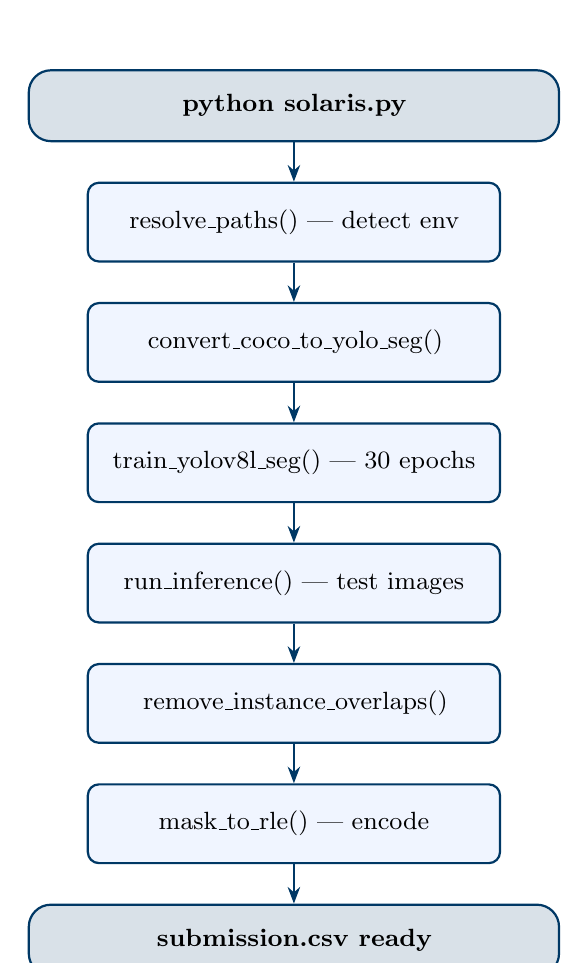
\begin{tikzpicture}[node distance=0.5cm]
  \node[term,text width=6.5cm](start){python solaris.py};
  \node[block,below=of start](rp){resolve\_paths() --- detect env};
  \node[block,below=of rp](conv){convert\_coco\_to\_yolo\_seg()};
  \node[block,below=of conv](train){train\_yolov8l\_seg() --- 30 epochs};
  \node[block,below=of train](infer){run\_inference() --- test images};
  \node[block,below=of infer](ovlp){remove\_instance\_overlaps()};
  \node[block,below=of ovlp](rle){mask\_to\_rle() --- encode};
  \node[term,below=of rle,text width=6.5cm](out){submission.csv ready};
  \foreach \a/\b in {start/rp,rp/conv,conv/train,
                     train/infer,infer/ovlp,ovlp/rle,rle/out}
    \draw[arrow](\a)--(\b);
\end{tikzpicture}
\caption{Complete execution flow of \texttt{solaris.py}.}
\label{fig:solaris_flow}
\end{figure}

\begin{table}[H]
\centering
\caption{Command-line modes of \texttt{solaris.py}.}
\renewcommand{\arraystretch}{1.3}
\begin{tabular}{l l p{6cm}}
\toprule
\textbf{Command} & \textbf{Mode} & \textbf{Action} \\
\midrule
\texttt{python solaris.py} & Full & Convert + Train + Predict \\
\texttt{python solaris.py --train} & Train only & Skip inference \\
\texttt{python solaris.py --predict --model best.pt} & Predict only & Skip training \\
\bottomrule
\end{tabular}
\label{tab:cli}
\end{table}

% ========================================================
\chapter{Results, Conclusion and Future Work}
% ========================================================

\section{Output Files}

\begin{table}[H]
\centering
\caption{Files produced by the Solaris pipeline.}
\renewcommand{\arraystretch}{1.3}
\begin{tabular}{l l p{7cm}}
\toprule
\textbf{File} & \textbf{Location} & \textbf{Contents} \\
\midrule
\texttt{best.pt}        & runs/yolov8l\_2048/weights/ & Best trained model weights \\
\texttt{last.pt}        & runs/yolov8l\_2048/weights/ & Final epoch weights \\
\texttt{submission.csv} & Working directory           & RLE predictions for Kaggle \\
\texttt{results.csv}    & Run directory               & Per-epoch training metrics \\
\bottomrule
\end{tabular}
\label{tab:outputs}
\end{table}

\section{Competition Result}

\textbf{Public Dice score: 0.55} --- achieved without ensembles, TTA, or hyperparameter
search. A strong baseline using a single model trained in one run.

\section{Advantages}

\begin{itemize}
  \item High resolution (2048px) preserves thin filament detail.
  \item Instance-level masks enable counting and shape analysis.
  \item Platform portability: zero code changes across environments.
  \item Mathematically guaranteed overlap-free predictions.
\end{itemize}

\section{Limitations and Future Work}

\begin{table}[H]
\centering
\caption{Recommended improvements and expected Dice gains.}
\renewcommand{\arraystretch}{1.3}
\begin{tabular}{c l l}
\toprule
\textbf{\#} & \textbf{Improvement} & \textbf{Expected Gain} \\
\midrule
1 & Test-Time Augmentation (TTA)    & $+0.01$--$0.03$ \\
2 & Multi-scale inference           & $+0.01$--$0.02$ \\
3 & Confidence threshold tuning     & $+0.01$--$0.02$ \\
4 & 80-epoch + cosine warm-up       & $+0.01$--$0.03$ \\
5 & YOLOv8x-Seg (extra-large)       & $+0.01$--$0.03$ \\
6 & Morphological closing           & $+0.005$--$0.01$ \\
\midrule
\textbf{Stacked} & All combined & $\sim$\textbf{0.60--0.65} \\
\bottomrule
\end{tabular}
\label{tab:future}
\end{table}

\section{Conclusion}

This project built an automated end-to-end pipeline for solar filament instance segmentation
using YOLOv8l-Seg. Implemented in a single script \texttt{solaris.py}, it covers every stage
from raw H-alpha image to a Kaggle-ready CSV.

Key achievements:
\begin{itemize}
  \item Platform-agnostic: Kaggle, Colab, local --- same code, zero changes.
  \item COCO-to-YOLO converter handling both polygon and RLE annotations.
  \item 2048px training preserving thin filament structure.
  \item Priority-based overlap-free instance masks.
  \item \textbf{Kaggle Dice score: 0.55} with no post-processing or ensemble.
\end{itemize}

This demonstrates that modern instance segmentation models, at appropriate resolution with
domain-adapted augmentation, can effectively automate solar filament detection --- a task
that historically required expert manual annotation.

\end{document}
